\documentclass[a4paper,11pt]{article}
\usepackage{amsmath}
\usepackage{xcolor}
\usepackage{soul}
\usepackage{graphicx}
\usepackage{geometry}
\usepackage{float}
\usepackage{hyperref}

\usepackage[labelfont=bf,skip=0pt]{subcaption}
\usepackage[labelfont=bf,skip=0pt]{caption}
\DeclareCaptionFormat{myformat}{\fontsize{8}{8}\selectfont#1#2#3}
\captionsetup{format=myformat}

\newcommand{\hlc}[2][yellow]{{%
    \colorlet{foo}{#1}%
    \sethlcolor{foo}\hl{#2}}%
}

\usepackage{titling}
\setlength{\droptitle}{-2cm}
\title{CombiFF}
\author{Salom\'e R. Rieder, Marina P. Oliveira, Philippe H. Hünenberger}
\date{}

\geometry{verbose,a4paper,tmargin=20mm,bmargin=20mm,lmargin=15mm,rmargin=15mm}

\begin{document}
\pagestyle{plain}
\maketitle

\newcommand{\vers}{\texttt{v\%\%}}
\newcommand{\fami}{\texttt{\#\#\#\#}}


%================================================================================
\section{\texttt{CombiFF} Workflow}
%================================================================================

The \texttt{CombiFF} workflow is illustrated in Figure \ref{cff_workflow}
%
\begin{figure}[h]
\begin{center}
  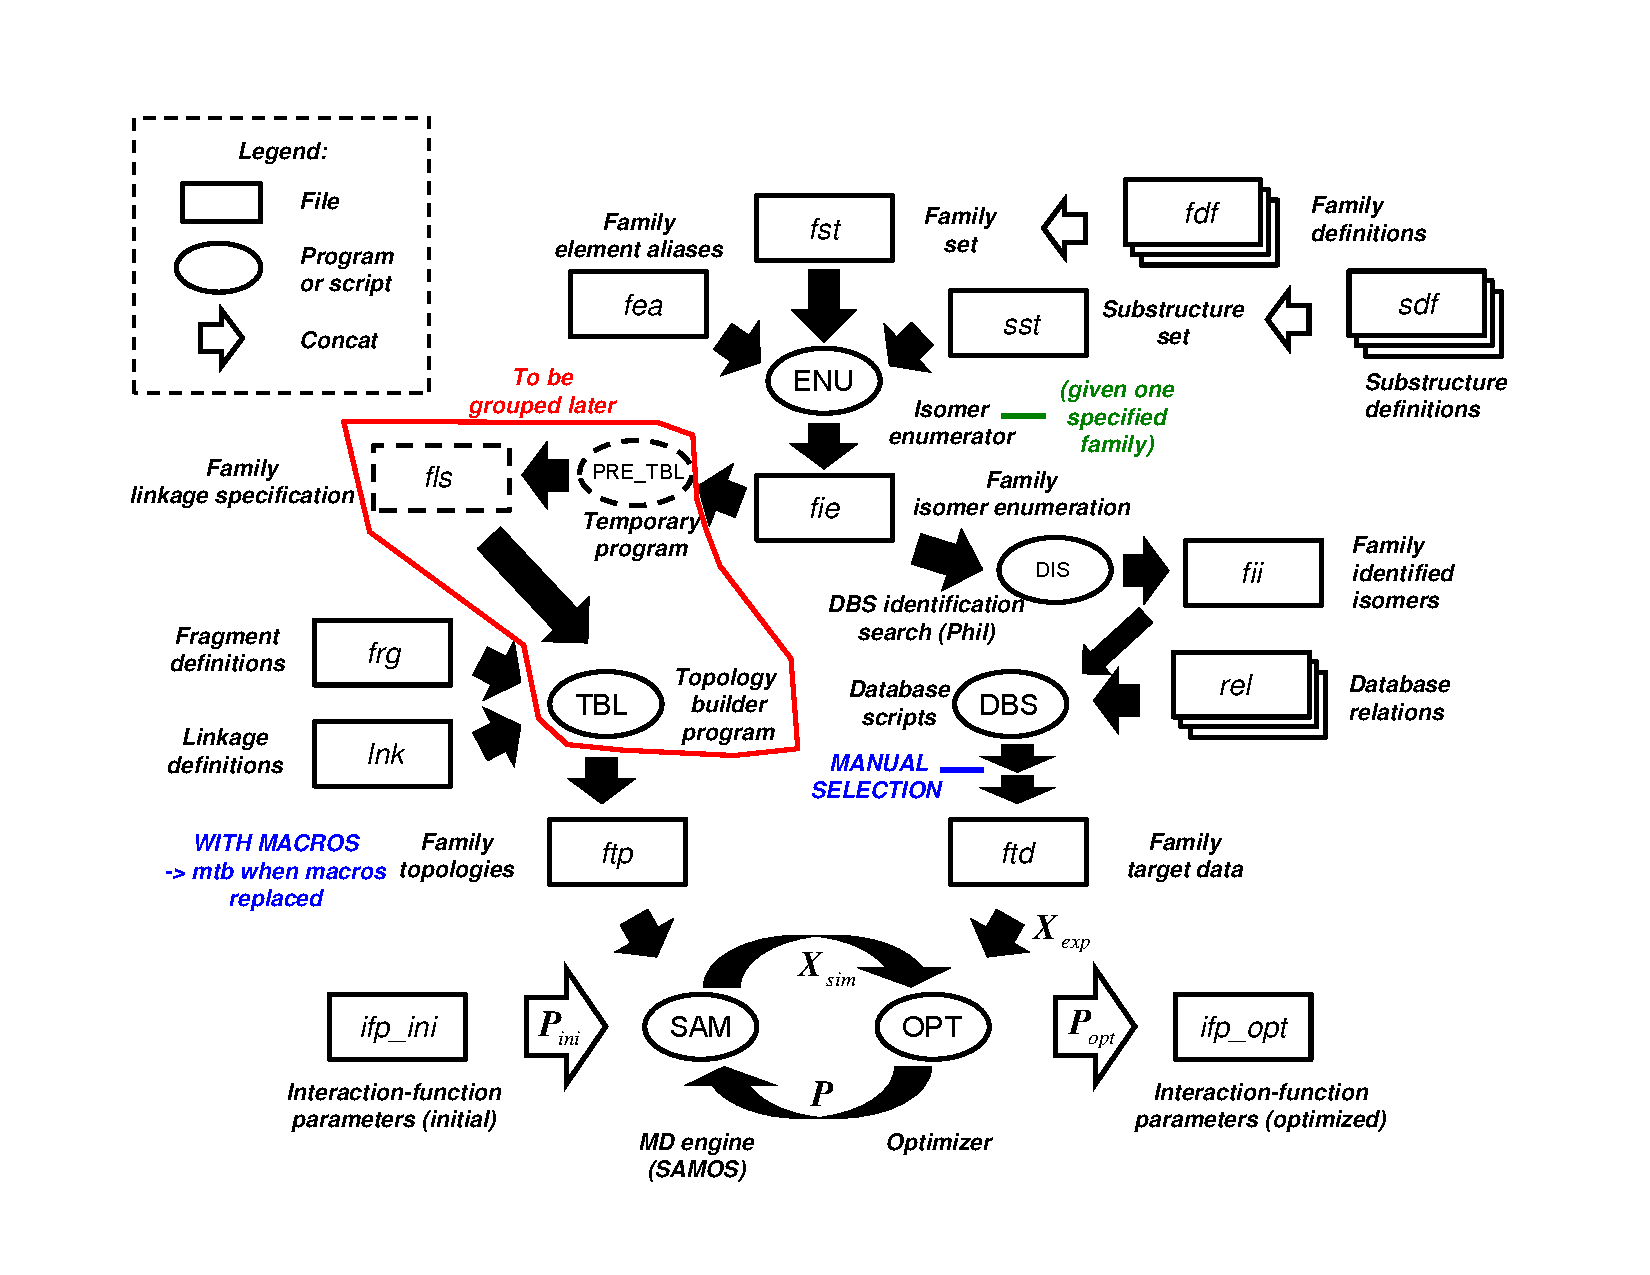
\includegraphics[clip=true,scale=0.6]{fig/cff_workflow.pdf}
\end{center}
\caption{XXX}
\label{cff_workflow}
\end{figure}
%

%================================================================================
\section{\texttt{CombiFF} Programs}
%================================================================================

The programs/scripts involved in \texttt{CombiFF} 
summarized in Table \ref{programs} and described 
in the following subsections.

\begin{table}[h!]
\begin{center}
\begin{tabular}{|l|l|}
\hline\hline
\multicolumn{2}{|c|}{Programs/scripts involved in \texttt{CombiFF}}\\
\hline
\texttt{enu} &  isomer enumerator \\
\texttt{tbl} &  topology builder \\
\texttt{DIS} &  (Phil-to-write) scans DBS to map \\
\texttt{DBS} &  scripts of the experimental database \\
\texttt{SAM} &  MD engine (SAMOS) \\
\texttt{OPT} &  parameter optimizer \\
\texttt{cnv} & converter and canonicalization program \\
\hline\hline
\end{tabular}
\end{center}
\caption{}
\label{programs}
\end{table}


%================================================================================
\section{\texttt{CombiFF} File Types}
%================================================================================

The file types involved in \texttt{CombiFF} 
summarized in Table \ref{file_types} and described 
in the following subsections.
%
For the labelling of the files, we will refer
to a version number (\vers) and to family numbers (\fami).
%
The family number is a four-digit number that refers to a given
family of compounds.
%

%--------------------------------------------------------------------------------
\subsection{Family definition file}
\label{filetype_fdf}
%--------------------------------------------------------------------------------

\begin{itemize}
\item Format: xml
\item Location: \texttt{CombiFF/use/input\_files/family\_definitions}
\item Content: specification of one or more compound families for enu 
\item Output of: Generated/edited manually
\item Input of: {\texttt{enu}}
\end{itemize}

A \texttt{fdf} file defines a given compound family with the number \fami\ within the \texttt{CombiFF} version \vers.
%
These files are created/edited manually to define/modify families.
%
\subsubsection{Format}
see \texttt{Combiff/use/input\_files/family\_definitions/README} and \texttt{Combiff/use/input\_files/family\_definitions/family\_definitions.dtd}


%--------------------------------------------------------------------------------
\subsection{Substructure files}
\label{filetype_sst}
%--------------------------------------------------------------------------------

\begin{itemize}
\item Format: xml
\item Location: \texttt{CombiFF/use/input\_files/substructures}
\item Content: substructures that can be included/excluded in the definition of families
\item Output of: Generated/edited manually
\item Input of: {\texttt{enu}}
\end{itemize}
%
\subsubsection{Format}
see \texttt{Combiff/use/input\_files/substructures/README} and \texttt{Combiff/use/input\_files/substructures/substructures.dtd}

%--------------------------------------------------------------------------------
\subsection{Alias files}\label{sec:filetype_ast}
%--------------------------------------------------------------------------------

\begin{itemize}
\item Format: xml
\item Location: \texttt{CombiFF/use/input\_files/aliases}
\item Content: aliases for sets of atom types (e.g. Hal for \{Br, Cl, F, I\}) that can be used in family definitions
\item Output of: Generated/edited manually
\item Input of: {\texttt{enu}}
\end{itemize}

\subsubsection{Format}
see \texttt{Combiff/use/input\_files/aliases/README} and \texttt{Combiff/use/input\_files/aliases/aliases.dtd}

%--------------------------------------------------------------------------------

\subsection{Pseudoatom files}\label{sec:filetype_pst}
\label{filetype_pst}
%--------------------------------------------------------------------------------

\begin{itemize}
\item Format: xml
\item Location: \texttt{CombiFF/use/input\_files/aliases}
\item Content: definition of pseudoatoms that can be used for family definitions
\item Output of: Generated/edited manually
\item Input of: {\texttt{enu}}
\end{itemize}

\subsubsection{Format}
see \texttt{Combiff/use/input\_files/pseudoatoms/README} and \texttt{Combiff/use/input\_files/pseudoatoms/pseudoatoms.dtd}

{
It is important to note that all atoms in a pseudoatom must be fully bonded, except for the atom in the first position of the ATOMS list. For example C-O-OH would be a valid pseudoatom, since only the carbon can form any bonds outside of the pseudoatom, but C-O-O would \emph{not} be a valid pseudoatom, since both the carbon and the 2nd oxygen can form bonds outside of the pseudoatom.
}

\subsection{Fragment files}
\label{filetype_frs}
\begin{itemize}
\item Format: xml
\item Location: \texttt{CombiFF/use/input\_files/fragments}
\item Content: definition of fragments to use to assemble molecules
\item Output of: Generated/edited manually
\item Input of: {\texttt{tbl}}
\end{itemize}

\subsubsection{Format}
see \texttt{Combiff/use/input\_files/fragments/README} and \texttt{Combiff/use/input\_files/fragments/fragments.dtd}

%--------------------------------------------------------------------------------
\subsection{Family isomer enumeration files}
\label{filetype_fie}
%--------------------------------------------------------------------------------

\begin{itemize}
\item Format: xml
\item Location: \texttt{CombiFF/use/output\_files/family\_isomer\_enumerations}
\item Content: list of constitutional isomers for a given family
\item Output of: \texttt{enu}
\item Input of: \texttt{tbl}
\end{itemize}

%--------------------------------------------------------------------------------

\subsection{Family stereoisomer enumeration files}
\label{filetype_fis}
%--------------------------------------------------------------------------------
\begin{itemize}
\item Format: xml
\item Location: \texttt{CombiFF/use/output\_files/family\_isomer\_enumerations\_stereo}
\item Content: list of stereoisomers (from tetrahedral centers and double bonds) for a given family
\item Output of: \texttt{enu}
\item Input of: --
\end{itemize}
%

\subsection{molecule decomposition files}
\label{filetype_fis}
%--------------------------------------------------------------------------------
\begin{itemize}
\item Format: xml
\item Location: \texttt{CombiFF/use/output\_files/molecule\_decompositions}
\item Content: specifies how to assemble the molecules of a family with given fragments
\item Output of: \texttt{tbl} or manual creation
\item Input of: \texttt{tbl}
\end{itemize}
%

\subsection{molecules with macros files}
\label{filetype_fis}
%--------------------------------------------------------------------------------
\begin{itemize}
\item Format: xml
\item Location: \texttt{CombiFF/use/output\_files/molecules\_with\_macros}
\item Content: molecular topologies with macro parameters for parameters (i.e. bond types, charges, etc.)
\item Output of: \texttt{tbl}
\item Input of: \texttt{tbl}
\end{itemize}

%--------------------------------------------------------------------------------
\subsection{GROMOS mtb files - with macros}
\label{filetype_mtb}
%--------------------------------------------------------------------------------

\begin{itemize}
\item Format: xml
\item Location: \texttt{CombiFF/use/output\_files/mtb}
\item Content: GROMOS mtb files for given families with macros
\item Output of: \texttt{tbl}
\item Input of: \texttt{tbl}
\end{itemize}

\subsection{GROMOS mtb files - with parameters}
\label{filetype_mtb}
%--------------------------------------------------------------------------------

\begin{itemize}
\item Format: xml
\item Location: \texttt{CombiFF/use/output\_files/mtb}
\item Content: GROMOS mtb files for given families with FF parameters
\item Output of: \texttt{tbl}
\item Input of: \texttt{GROMOS/SAMOS}
\end{itemize}



\end{document}



